\documentclass[a4paper,10pt]{article}
\usepackage[utf8]{inputenc}
\usepackage{graphicx}
\usepackage{url}
\usepackage{float}
\usepackage{times}
\usepackage{multirow}
\usepackage{listings}
\usepackage{times}
\usepackage{paralist}
%\usepackage{epsfig}
\usepackage[figtopcap]{subfigure}
\usepackage[hypertex]{hyperref}
\usepackage{subfigure}
\usepackage{color}


%\documentclass{rspublic}

\usepackage{ifpdf}


\newif\ifdraft
\drafttrue
\ifdraft
\newcommand{\jhanote}[1]{ {\textcolor{red} { ***shantenu: #1 }}}
\newcommand{\alnote}[1]{ {\textcolor{blue} { ***andre: #1 }}}
\newcommand{\athotanote}[1]{ {\textcolor{green} { ***athota: #1 }}}
\else
\newcommand{\alnote}[1]{}
\newcommand{\jhanote}[1]{}
\newcommand{\athotanote}[1]{}
\fi

\newcommand{\I}[1]{\textit{#1}}
\newcommand{\B}[1]{\textbf{#1}}
\newcommand{\BI}[1]{\textbf{\textit{#1}}}
\newcommand{\T}[1]{\texttt{#1}}

\setlength\topmargin{0in}
\setlength\headheight{0in}
\setlength\headsep{0in}
\setlength\textheight{9in}
\setlength\textwidth{6.5in}
\setlength\oddsidemargin{0in}
\setlength\evensidemargin{0in}
\setlength\parindent{0.1in}
\setlength\parskip{0.25em}


\ifpdf
  \DeclareGraphicsExtensions{.pdf, .jpg}
 \else
  \DeclareGraphicsExtensions{.eps, .ps}
\fi

\newcommand{\note}[1]{ {\textcolor{red} { ***NOTE: #1 }}}

\begin{document}

\title{\LARGE Running Asynchronous Replica-Exchange Simulations Across Heterogeneous Distributed Infrastructures}
 
\author{Abhinav Thota$^{1,2}$, Andre Luckow$^{1}$, Shantenu Jha$^{1,2,3}$\\
   \small{\emph{$^{1}$Center for Computation \& Technology, Louisiana State University, USA}}\\
   \small{\emph{$^{2}$Department of Computer Science, Louisiana State University, USA}}\\
   \small{\emph{$^{3}$e-Science Institute, University of Edinburgh, UK}}
   }
 
\maketitle

\section{Introduction}
 
Developing applications that are able to orchestrate heterogeneous
resources across distributed resources is a complex task.  Inevitably,
the design and development of an applicaiton is influenced and
constrained by the programming systems and the infrastructure it is
developed against. Breaking this coupling between the development and
the underlying infrastructure, to enable applications to be flexible
(across infrastructure), extensible (to new methods of communiction
and coordination) and scalable is an important design objective of
distributed applications -- both logically distributed and physically
distributed.

In this work, we focus on the Replica-Exchange (RE)
~\cite{hansmann,Sugita:1999rm} Methods -- which represent a class of
algorithms that involve a large number of loosely-coupled ensembles.
RE simulations are used to understand physical phenomena -- ranging
from protein folding dynamics to binding affinity calculations.

In this work, we develop a flexible, extensible and scalable
implementation of RE that can utilise a range of infrastructure
concurrently (and autonomically/adaptively), that supports different
coordination mechanisms (publish-subscribe, centralised notification),
different replica pairing mechanisms (synchronous versus asynchronous)
and thereby different variants of the RE algorithm. We implement and
demonstrate how flexible and robust implementation enables the
effecient use of a broad range of infrastructure.

% Several classes of applications, which are well suited for loosely
% coupled Grids, exist; that belongs to this category are
% \emph{Replica Exchange (RE)} simulations.  1 para intro to
% replica-exchange, and how it is traditionally done (ie case I)

\section{Replica-Exchange Approach}

The RE algorithm involves the concurrent execution of multiple similar
simulations, the \emph{replicas}.  There is a loose-coupling between
the replicas in form of periodic exchange attempts between paired
replicas. Previously, we demonstrated the usage of the SAGA Pilot-Job
framework~\cite{saga_bigjob_condor_cloud} -- called the BigJob, to run
replica exchange simulations across multiple, heterogeneous
distributed Grid and Cloud infrastructures~\cite{Luckow:2008fp}.
\alnote{maybe we should also intro SAGA at some point} \jhanote{Yes}
The Simple API for Grid Applications (SAGA) is an
API standardization effort within the Open Grid Forum
(OGF) ~\cite{}, an international standards development body
concerned primarily with standards for distributed computing.
Further, we introduced several adaptivity modes, e.\,g.\ adaptive
sampling that are able to react to dynamic changes in resource
availabilities.

\alnote{Not sure how many technical we need to provide...}  Depending
on the number of processes \texttt{N}, the manager creates \texttt{N/2} pairs
of replicas.  Before launching a job, the manager ensures that all
required input files are transferred to the respective resource. For
this purpose, the SAGA File API and the GridFTP adaptor are used. The
replica jobs are then submitted to the resource using the SAGA CPR
API and the MIGOL/GRAM middleware.

For the vanilla implementation of RE(Case I), when the replicas reach a
pre-determined state (e.g. the NAMD job finishes after a fixed number
of steps), a decision as to whether to exchange temperatures between
previously paired replicas is determined using the Metropolis scheme.
The run of an ensemble of replicas in parallel and the subsequent
pairwise exchange attempt are referred to as generation. No two
replicas can belong to different generations. If the exchange attempt
is successful, parameters such as the temperature are swapped. Both
jobs are then relaunched.  \athotanote{I have tried to put here how
  the adaptive repex was done, supposing that it was case 1. Or should
  a general explanation of a replica exchange be here?} \jhanote{I
  think this is ok}
 
% 1 para limitation on traditional replica exchange
The major limitation of this model is that the replicas are paired and that exchanges can only take place between the paired replicas. 
This limits the group of replicas which are available for exchange. Moreover, the replicas are attached to their partners, 
sometimes waiting for them to complete while there are possibly other replicas available which are paired to their partners.
This puts a strain on the number of exchanges that can take place within a certain time.  \athotanote{is it better to have a wide group of replicas?
  need some input here!}

\jhanote{The point is really the following: Paired-replicas are Ok if
  it can be guaranteed that equal resources will be available, or the
  resource availabilty can be predicted in advance. However, in
  distributed systems, whereby definition, resource availability
  fluctates it is important to have a scheme/implementation that does
  not depend on a static, well-defined model of resource availability
  and execution. This forms the motivation for coming up with a
  formulation of a well known algorithm that makes it suitable for a
  range of infrastruture.}
  

  
\subsection{Asynchronous Replica Exchange}
%- Introduce asynchronous Replica Exchange --  1 para on case II and case III (algorithmically)

To overcome these limitations we propose an asynchronous replica
exchange algorithm similar to Parashar et al.~\cite{parashar_arepex}
where replicas can perform exchanges asynchronously. The possibility
to conduct exchanges asynchronously also eliminates the need to limit
exchanges to fixed pairs of replicas and allows exchanges with any
other replica available.
 
\alnote{We need to highlight how we particularly differ from Parashar
  et al: no comet, no MPI jobs, production Grids, understand
  performance sentence...}

The asynchronous replica exchange framework builds upon the SAGA BigJob and RE frameworks discussed previously.
We present two variants of the Asynchronous RE algorithm. The first is a centralized 
mechanism where all the replicas are managed by a master. The master will closely monitor the replicas and will make the exchanges when feasible. 
The second is a decentralized mechanism where each replica is managed individually and independently. An agent is launched in place of the replica and will perform the the required actions on behalf of the replica.
%Describe how we implement Case II and Case III (you can use figures)
%using SAGA and the advantages


\subsubsection{Centralized Asynchronous RE}

%%%%% FIGURE %%%%%
\begin{figure}
\centering
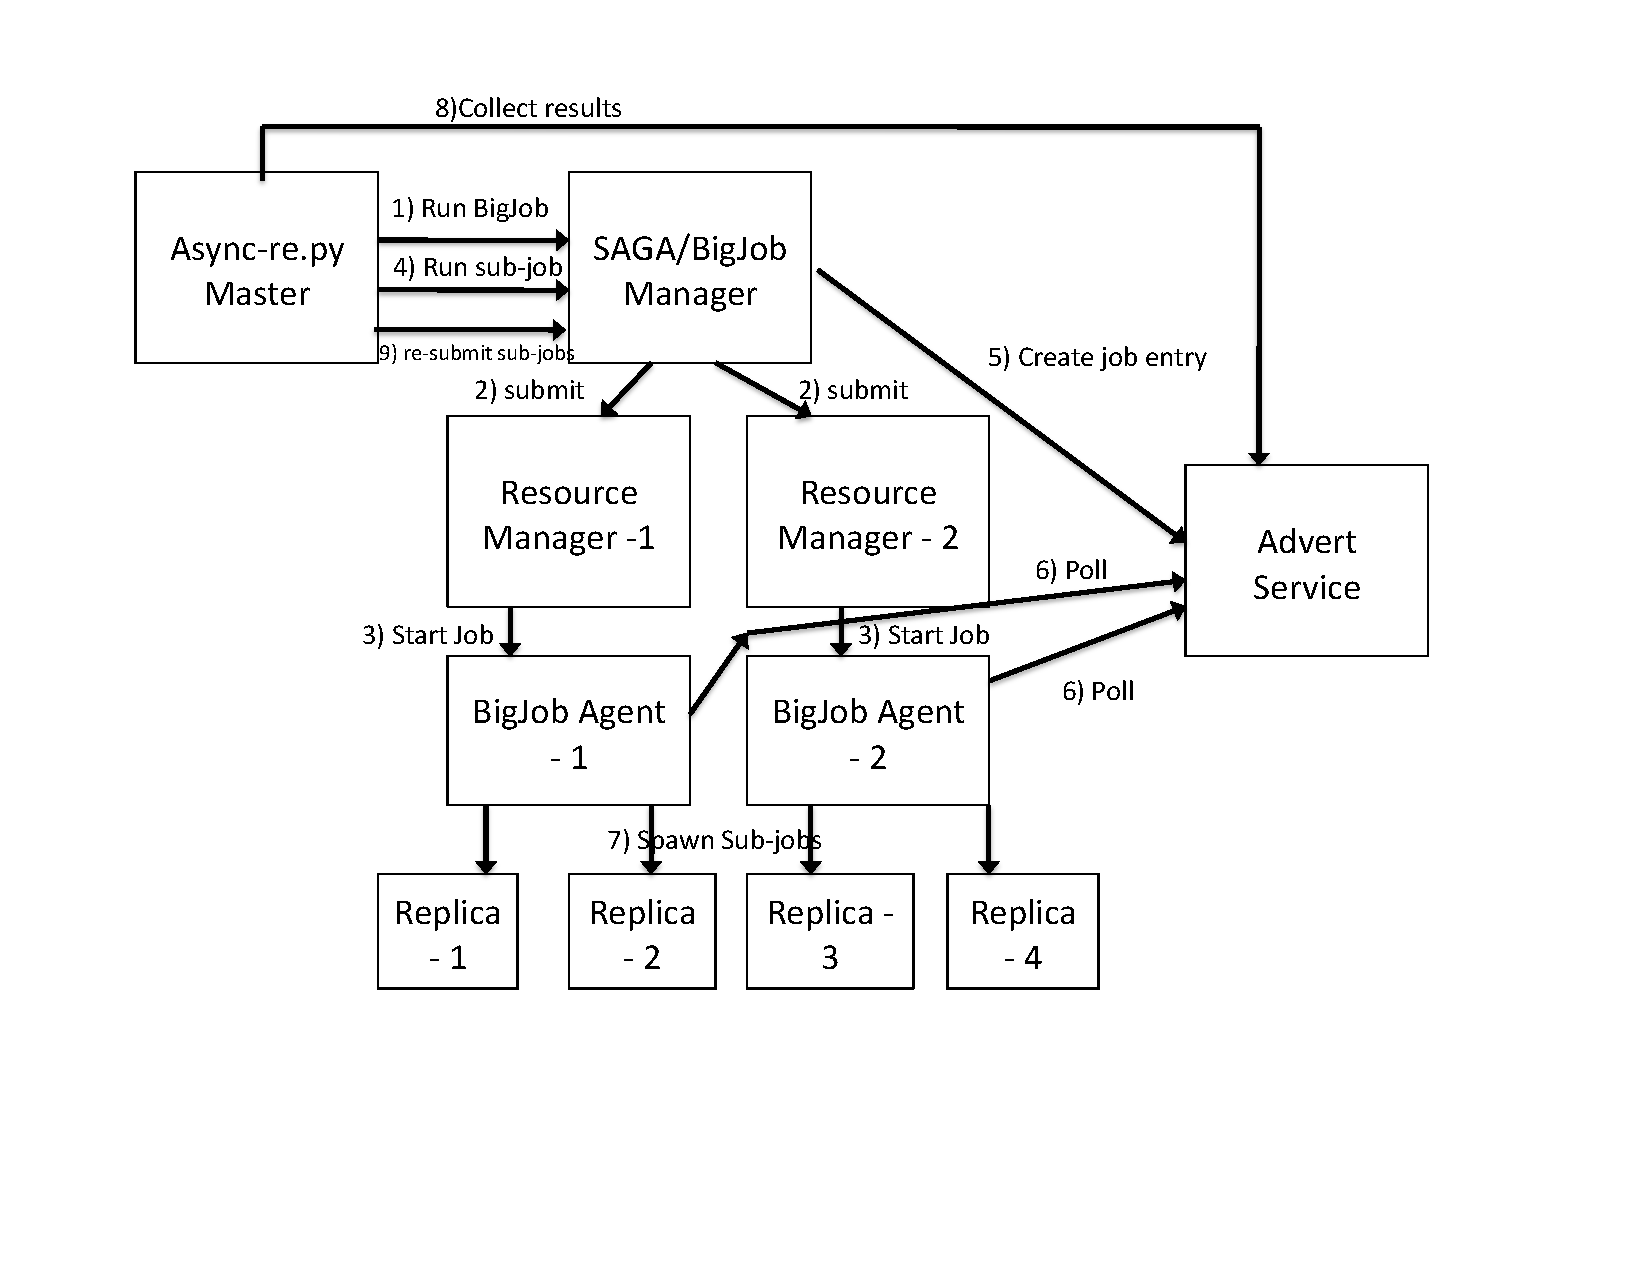
\includegraphics[scale=0.50]{figures/centralized_architecture}
\caption{\small Centralized Asynchronous Replica Exchange}
\label{fig:centralized}
%\vspace{-1em}
\end{figure}

In the case of the centralized version of the asynchronous replica exchange(Case II), one or more BigJobs are
launched and the replicas are submitted to the BigJobs as and when they become active. The master, which also launches the BigJob,
now monitors the replicas. When a replica is in done state, the master will start a search for an appropriate partner from all the available replicas. The decision as to make the exchange or not is made using the Metropolis scheme. 
Whether or not a successful exchange takes place, the master again monitors all the replicas and  repeats the steps mentioned.
After each successful exchange the replicas are resubmitted to the BigJob(s) and restarted.

\subsubsection{Decentralized Asynchronous RE}

%%%%% FIGURE %%%%%
\begin{figure}
\centering

\subfigure[Overall Architecture]{
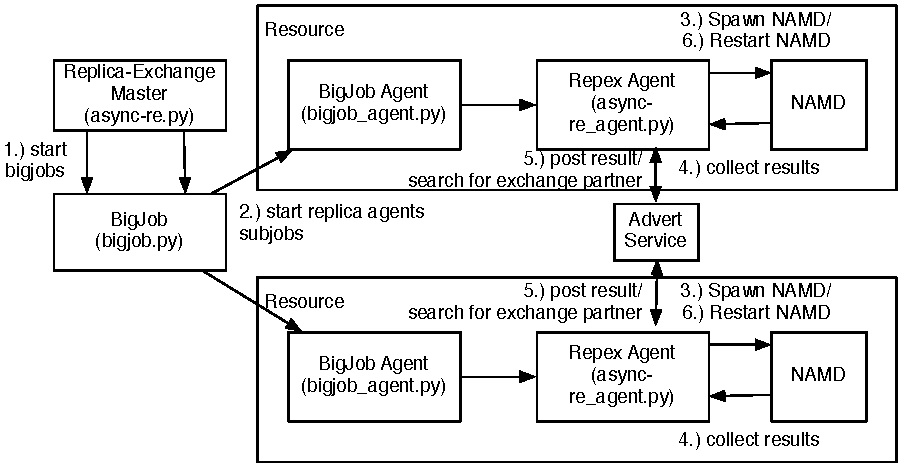
\includegraphics[width=0.57\textwidth]{figures/decentralized_architecture.pdf}
\label{fig:subfig2}
}
\subfigure[Control Flow: Replica Exchange]{
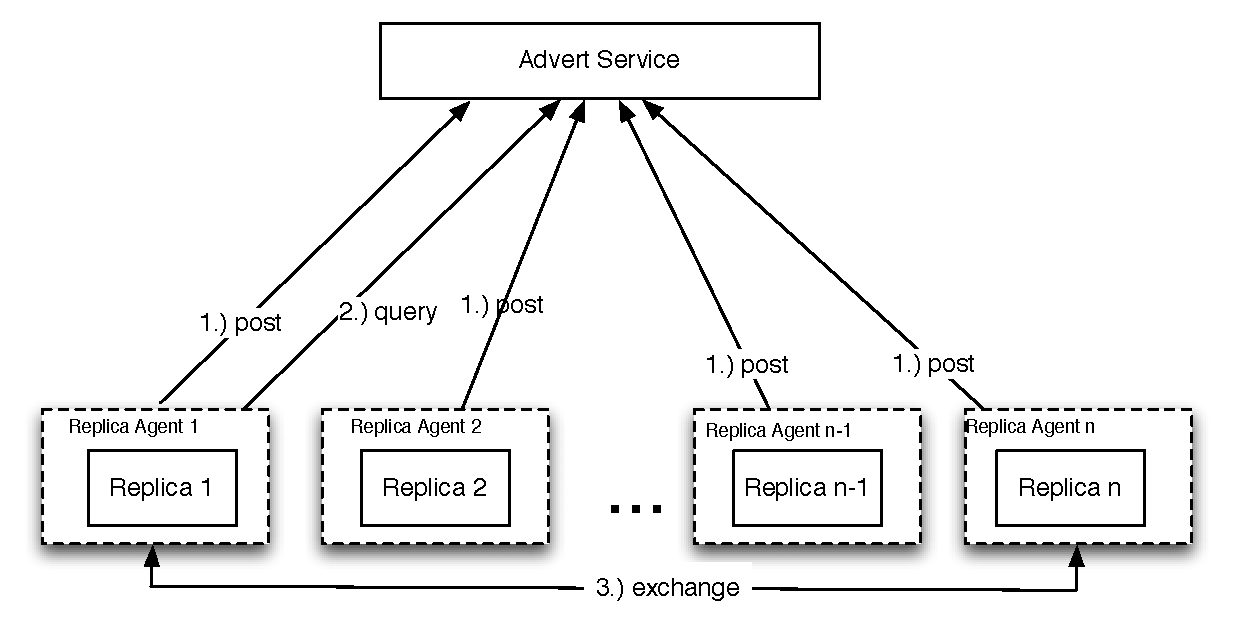
\includegraphics[width=0.35\textwidth]{figures/asyncre.pdf}
\label{fig:subfig1}
}

% 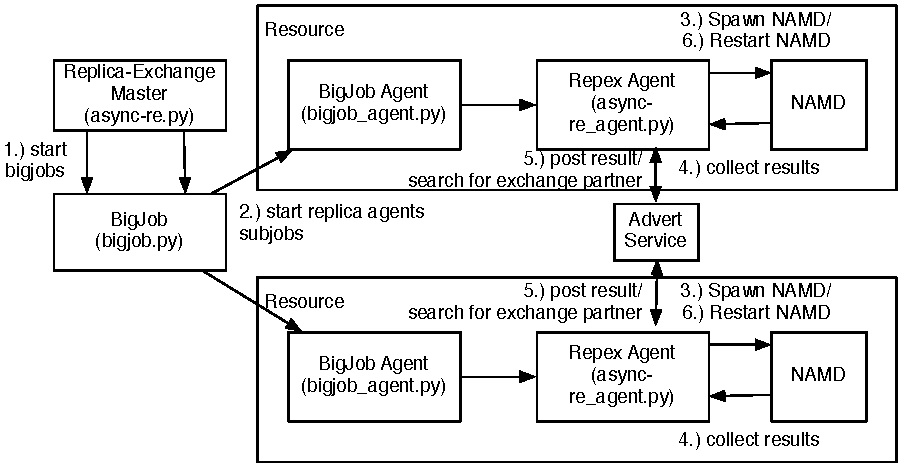
\includegraphics[scale=0.50]{figures/decentralized_architecture.pdf}
\caption{\small Decentralized Asynchronous Replica Exchange}
\label{fig:decentralized}
%\vspace{-1em}
\end{figure}
%%%%% FIGURE %%%%%

Case III is the decentralized version. In this version, one or more BigJobs are launched but instead of submitting the replicas as sub-jobs, an agent is launched in place of the replica. The agent is nothing but a wrapper script for the replica. The script then runs the replica and monitors the replica and looks for partners to exchange as and when the replica is ready. In this case the various functions needed to make the exchange are carried out by the wrapper script. The temperatures, energies and states of a replica are reported to and retrieved from the SAGA advert service in real-time.
\jhanote{The distinction between
  Case 3 and 2 needs to be made more clear. The following is
  ``implementation detail''. What is the conceptual difference between
  Case 3 and Case 2?} 

\section{Conclusion}
With an asynchronous replica exchange mechanism we can improve the number of exchanges per unit time, 
a key parameter in judging the performance of a replica-exchange mechanism. \athotanote{is this right? } 
We are also going to have a wider group of replicas to look at for each replica as we are not pairing 
the replicas. Also, we have the usual advantages of using a pilot-job, such as reduced queue wait 
times by not having to submit to the queue. 
We also provide major advantages when compared to Parashar et al. We are using Teragrid and LONI resources to run the asynchronous replica exchange simulations. We also have the ability to run MPI jobs. We need to evaluate the performance of our models and compare with other models for conducting replica exchange simulations. 

Unfortunately we have results only for Case II, but we will establish the ability to scale-out across different infrastructure. We will provide a comparison of the performance of the asynchronous RE versus the synchronous RE at unprecedented scales. Lastly, we will compare the two different implementations of the asynchronous replica exchange.


%With this asynchronous replica exchange mechanism we can improve the
%number of exchanges per unit time, a key parameter in judging the
%performance of a replica-exchange mechanism. \athotanote{is this
 % right? }  We are also going to have a wider group of replicas to
%look at for each replica as we are not pairing the replicas. Also, we
%have the usual advantages of using a pilot-job, such as reduced queue
%wait times by not having to submit to the queue.  Unfortunately we
%dont have results \jhanote{What results can we present -- any? some?},
%so we will say, (i) we establish the ability to scale-out (distributed
%and exa-scale) across different infrastructure (ii) compare the Async
%versus sync formulation at unprecedented scales \jhanote{At least
%  outline what infrastructure we / you are planning to use?} (iii)
%compare different implementations of the Async version
 
 \bibliographystyle{IEEEtran} 
 \bibliography{literature,saga}


\end{document}

